\documentclass{beamer}
\usepackage{animate}
\usepackage{amsmath}
\usepackage{braket}
\usepackage{caption}
\usepackage{subcaption}
\usepackage[utf8]{inputenc}
\usepackage{csquotes}
\usepackage[english]{babel}
\usepackage{tikz-cd}
\usepackage[
  backend=biber,
  style=numeric,
  citestyle=numeric,
  sorting=none
]{biblatex}
\addbibresource{refs.bib}

\setbeamertemplate{bibliography item}{\insertbiblabel}

\usetheme{Boadilla}

\captionsetup{font=tiny,labelfont=tiny}

\title{Quantum Computing}
\subtitle{From Zero to Giving-up}
\author{Ming Lu}
\date{\today}


\begin{document}

\begin{frame}
  \titlepage
\end{frame}

\begin{frame}
  These sslides are notes when reading book
  \newline
  \newline
  \LARGE{\textrm{Quantum Computing: A Gentle Introduction}}\tiny\cite{gentleintroduction}
  \newline
  \newline
  \small{\textrm{Eleanor Rieffel and Wolfgang Polak}}
\end{frame}

\begin{frame}{Bibliography}
  \AtNextBibliography{\tiny}
  \printbibliography
\end{frame}

\begin{frame}{Outline}
  \tableofcontents
\end{frame}

\section{The Quantum Mechanics}
\begin{frame}
  The Quantum Mechanics
\end{frame}

\subsection{Quantum Particles}
\begin{frame}
  \frametitle{Quantum Particles}
  \begin{columns}
    \column{0.6\textwidth}
    Think a partical as a wave in some field.
    What human-beings are able to sense are only differences/waves in these fields.\tiny\cite{quantumparticle}
    \column{0.4\textwidth}
    \begin{figure}
      \animategraphics[loop,autoplay,width=\linewidth,keepaspectratio]
      {24}
      {figures/quantum-particle-electron-photon/quantum-particle-electron-photon-}
      {0}
      {129}
      \caption{Electron and Photon. Source: Fermilab}
    \end{figure}
  \end{columns}
\end{frame}


\subsection{Photon Polarization Experiment}
\begin{frame}
  \frametitle{Photon Polarization Experiment}
  \begin{figure}
    \centering
    \begin{subfigure}[b]{0.3\textwidth}
      \centering
      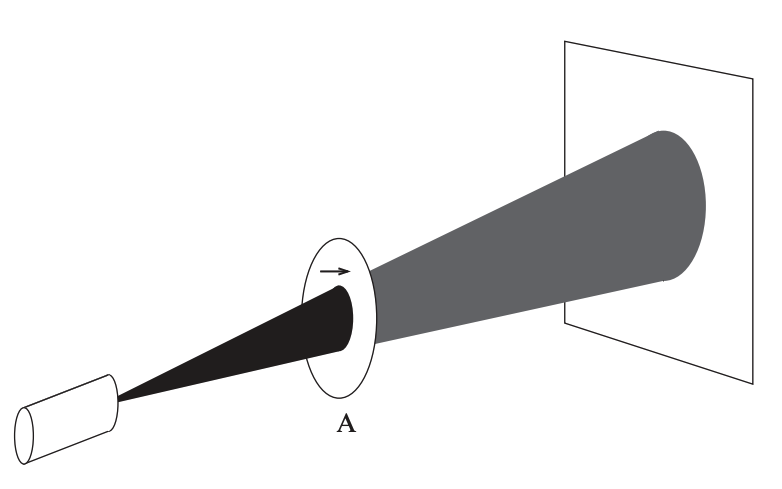
\includegraphics[scale=0.12]{figures/polarization-0}
      \caption{polaroid A with preferred axis $\ket{\rightarrow}$}
      \label{fig:polarization-0}
    \end{subfigure}
    \hfill
    \begin{subfigure}[b]{0.3\textwidth}
      \centering
      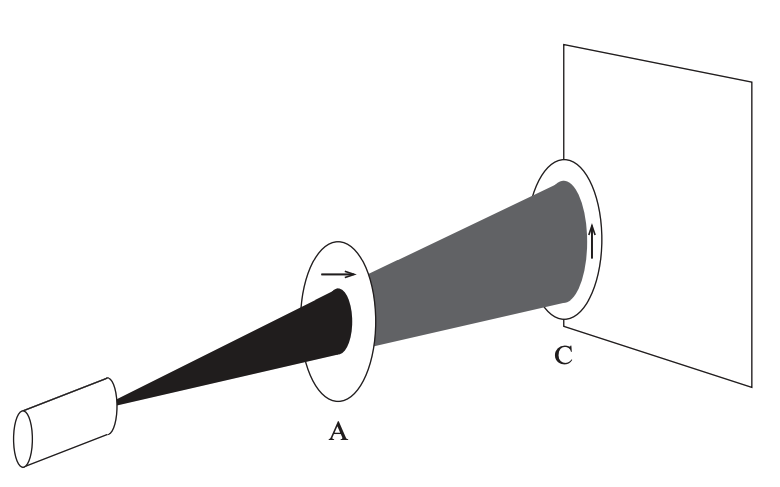
\includegraphics[scale=0.12]{figures/polarization-1}
      \caption{polaroid C with preferred axis $\ket{\uparrow}$}
      \label{fig:polarization-1}
    \end{subfigure}
    \hfill
    \begin{subfigure}[b]{0.3\textwidth}
      \centering
      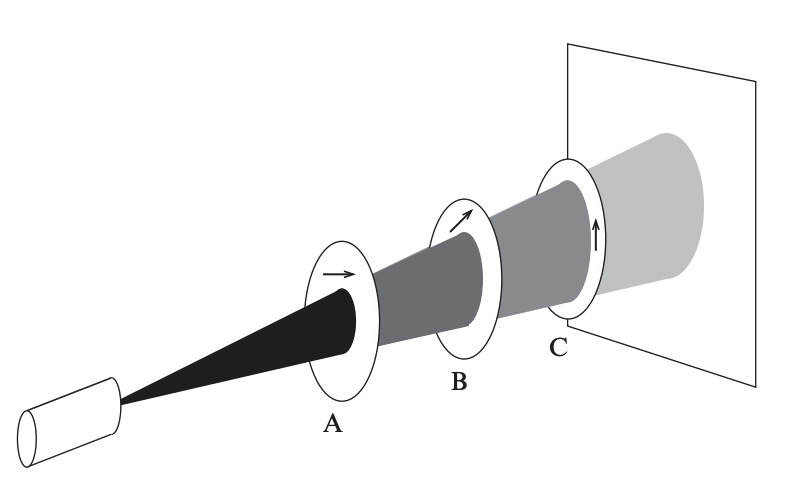
\includegraphics[scale=0.12]{figures/polarization-2}
      \caption{polaroid B with preferred axis $\ket{\nearrow}$}
      \label{fig:polarization-2}
    \end{subfigure}
    \caption{Photon Polarization Experiment\tiny\cite{gentleintroduction}}
    \label{fig:Polarization-3}
  \end{figure}

  \begin{block}{An explanation from quantum mechanics}
    Model a photon (a qubit) as a vector in a 2-dimensional vector space:
    $\ket{v} = a\ket{\uparrow}+ b\ket{\rightarrow}$,
    where $|a|^{2}+|b|^{2}=1$ and \{$\ket{\uparrow}$ and $\ket{\rightarrow}$\} is a basis of the vector space.
    \par
    A polaroid with preferred axis $\ket{\uparrow}$ (like C in figure) can:
    \begin{enumerate}[I]
      \item allow the photon get through with \textbf{possibility} $|a|^2$
      \item absorb the photon with \textbf{possibility} $|b|^2$
      \item polarized the passed photon in direction of $\ket{\uparrow}$
    \end{enumerate}
  \end{block}
\end{frame}

\subsection{Impact of Measurement}
\begin{frame}
  \frametitle{Impact of Measurement}
  \begin{columns}
    \column{0.37\textwidth}
    \begin{figure}
      \centering
      \begin{subfigure}[b]{0.45\textwidth}
        \centering
        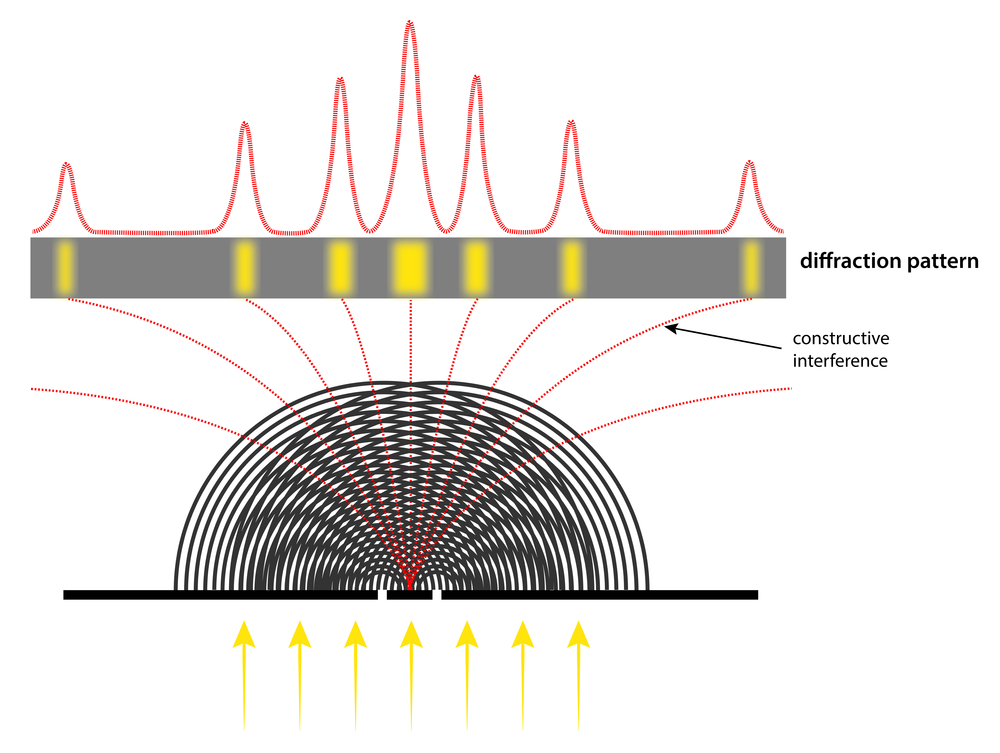
\includegraphics[scale=0.3]{figures/double-slit-0}
        \caption{Double-Slit w/o Detector}
        \label{fig:doube-slit-0}
      \end{subfigure}
      \hfill
      \begin{subfigure}[b]{0.45\textwidth}
        \centering
        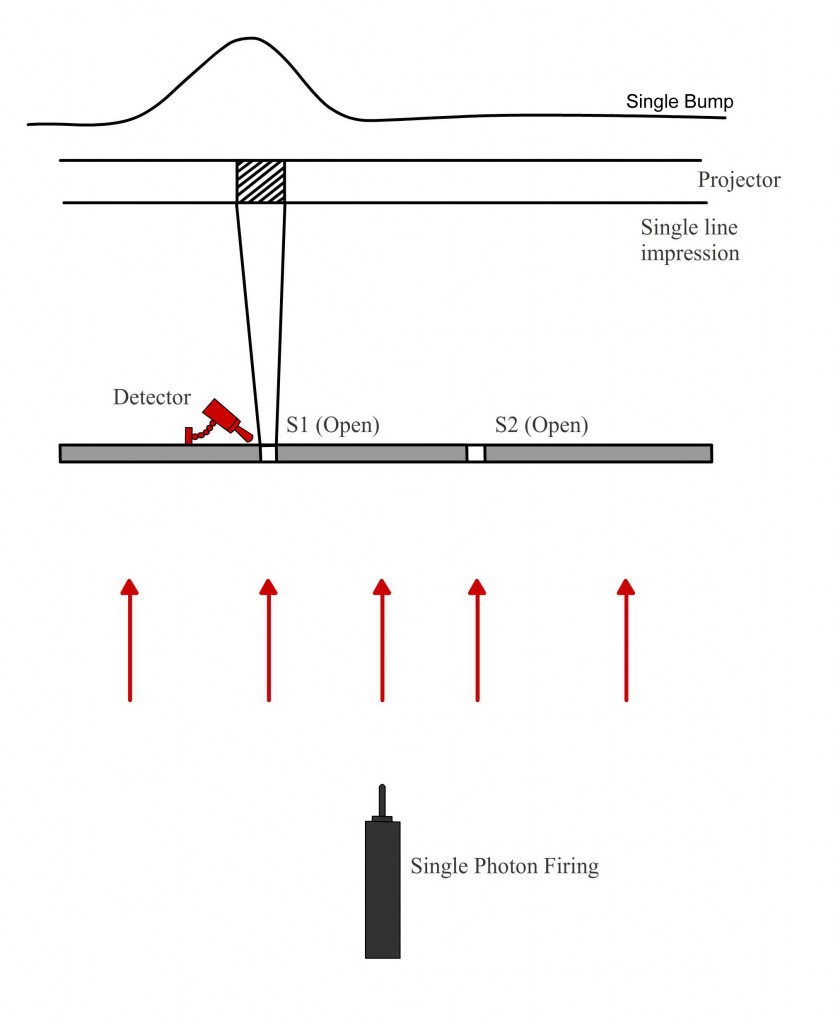
\includegraphics[scale=0.075]{figures/double-slit-1}
        \caption{Double-Slit w/ Detector}
        \label{fig:doube-slit-1}
      \end{subfigure}
      \caption{Double-Slit Experiment\tiny\cite{doubleslit}}
      \label{fig:doube-slit-2}
    \end{figure}
    \begin{figure}
      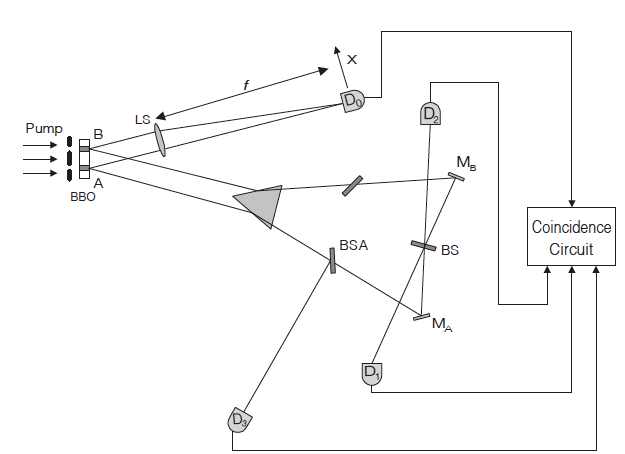
\includegraphics[scale=0.155]{figures/delayed-choice-quantum-eraser}
      \caption{Delayed Choice Quantum Eraser\tiny\cite{delayed}}
    \end{figure}

    \column{0.63\textwidth}
    \begin{block}{Measurement}
      A qubit
        \begin{align*}
        \ket{v} &= a\ket{\uparrow}+ b\ket{\rightarrow} \\
                &= x\ket{\nwarrow}+ y\ket{\nearrow}
        \label{eqn:qubit-bases}
        \end{align*}
      \begin{enumerate}[I]
        \item must be measured in one certain basis, e.g. \{$\ket{\uparrow}$ and $\ket{\rightarrow}$\},
          or \{$\ket{\nwarrow}$ and $\ket{\nearrow}$\};
          the result of measurement is in \textbf{possibility}, which is caused by \textbf{superposition} of the states in a basis.
        \item can be measured once and only once; after being measured, it gives \textbf{deterministic} result, as the quantum system in it has \textbf{decoherented}.
      \end{enumerate}
    \end{block}
  \end{columns}
\end{frame}

\subsection{BB84}
\begin{frame}{BB84: A Quantum Key Distribution Protocol}
  \framesubtitle{The Problem}
  Bob and Alice want to share some secret bits (key). They don't want Eve to know the secret bits.
  \setbeamerfont{block title}{size=\scriptsize}
  \begin{block}{What Bob and Alice can do:}
  {\scriptsize
    \begin{enumerate}[I]
      \item A classical channel to transfer bits.
      \item A quantum channel to transfer qubits.
      \item Encode and measure qubits with Standard basis $\ket{\uparrow}$ and $\ket{\rightarrow}$.
      \item Encode and measure qubits with Hadamard basis $\ket{\nearrow}$ and $\ket{\nwarrow}$.
    \end{enumerate}
  }%
  \end{block}
  \begin{block}{What Eve can do:}
  {\scriptsize
    \begin{enumerate}[I]
      \item Eavesdrop on classical channel.
      \item Eavesdrop a qubit from quantum channel and send another qubit to Bob.
      \item Encode and measure qubits with Standard basis $\ket{\uparrow}$ and $\ket{\rightarrow}$.
      \item Encode and measure qubits with Hadamard basis $\ket{\nearrow}$ and $\ket{\nwarrow}$.
    \end{enumerate}
  }%
  \end{block}
\end{frame}

\begin{frame}{BB84: A Quantum Key Distribution Protocol}
  \setbeamerfont{block title}{size=\scriptsize}
  \begin{block}{How it works}
  {\scriptsize
    \begin{enumerate}[I]
      \item Alice encodes a bit into a qubit with one basis and sends it to Bob through quantum channel;
      \item Eve eavesdrops the qubit and meansures it by \textbf{randomly} picking a basis since she doesn't know the basis Alice used; and then encodes/clones the result into a new qubit with the picked basis and sends it to Bob;
      \item Bob meansures the qubit by randomly picking a basis as well;
      \item through classical channel, Bob tells Alice that the qubit has been received;
      \item through classical channel, Bob and Alice exchange the bases they used;
      \item if they same basis, the result bit by measuring the qubit is kept as one basis-matching bit;
      \item else, the result is dropped;
      \item continue steps above until Bob and Alice have enough basis-matching bits;
      \item Bob and Alice agree to select half from those basis-matching bits, and exchange the values of these bits through classical channel;
      \item if there are \textbf{unmatched values}, they are sure about that Eve is eavesdroping;
      \item if there are no unmatched values, it's probably safe to use remaining half of basis-matching bits as final secret bits (key).
    \end{enumerate}
  }%
  \end{block}
\end{frame}

\begin{frame}[fragile]{BB84: How secure the secure bits are?}
  \begin{tikzcd}[row sep=tiny]
    & & & & & & 90 \\
    & & & & 100 \ar[urr, sloped, "matched"] \ar[drr, sloped, "unmatched"] \\
    & & 200 \ar[drr, sloped, "secure\ bits?"] \ar[urr, sloped, "value\ verifying"] & & & & 10 \\
    400 \ar[urr, sloped, "basis\ matched"] \ar[drr, sloped, "basis\ unmatched"'] & & & & 100 \\
    & & 200
  \end{tikzcd}

  \setbeamerfont{block title}{size=\scriptsize}
  \begin{block}{Why there are unmatched values?}
    {\scriptsize
      Because Eve doesn't know the basis Alice used to encode the qubit, she has to pick one basis \textbf{randomly} to encode/clone the qubit again. 
      When Eve picked wrong basis, Bob's measurement would get unmatched value in \textbf{possibility}.
      \par
      Can you calculate the possibility exactly?
      \begin{align*}
        \ket{\nearrow} =& \frac{1}{\sqrt{2}}(\ket{\uparrow} + \ket{\rightarrow}) \\
        \ket{\nwarrow} =& \frac{1}{\sqrt{2}}(\ket{\uparrow} - \ket{\rightarrow})
      \end{align*}
    }%
  \end{block}
\end{frame}

\section{Single Qubit System}
\begin{frame}
  Single-Qubit System
\end{frame}
\subsection{Basis}
\begin{frame}{Basis}
  {\tiny
    All possible states of a one-qubit (quantum) system is viewed as a two-dimensional complex vector space. One state can be denated as a vector $\ket{\psi}$ in this space:
  \begin{align*}
    \ket{\psi}&=\alpha\ket{0}+\beta\ket{1} \\
              &=\alpha\begin{bmatrix}1\\0\end{bmatrix}+\beta\begin{bmatrix}0\\1\end{bmatrix}
  \end{align*}
  with \textbf{complex numbers} $\alpha$ and $\beta$, and the normalization constraint $\braket{\psi|\psi}=1$.
  \par
  The $\ket{0}$ and $\ket{1}$, which can be any one pair of \textbf{orthonormal} vectors in this vector space, is a \textbf{basis}.
  }%
\end{frame}

\subsection{Bloch Sphere}
\begin{frame}{State of Single-Qubit System\tiny\cite{blochsphere}}
  \framesubtitle{From 2-Dimensional Complex Vector Space to 3-Dimensional Real Space}
  {\tiny
  A single qubit can be written as:
  \begin{columns}
  \column{0.65\textwidth}
  \begin{align*}
    \ket{\psi} &= \alpha\ket{0}+\beta\ket{1} \\
               &= r_{\alpha}(\cos\phi_{\alpha} + i\,\sin\phi_{\alpha})\ket{0}+\beta\ket{1} \\
               &= r_{\alpha}e^{i\phi_{\alpha}}\ket{0} + r_{\beta}e^{i\phi_{\beta}}\ket{1}
    \\
    e^{-i\phi_{\alpha}}\ket{\psi} &= r_{\alpha}\ket{0} + r_{\beta}e^{i\phi}\ket{1} \\
                                  &= r_{\alpha}\ket{0} + (x+i\,y)\ket{1} \\
                                  &= \ket{\psi'}
  \end{align*}
  $e^{-i\phi_{\alpha}}$ is a \textbf{global phase}, which has no observable consequences.
  \begin{align*}
    \braket{\psi'|\psi'} &= 1 \\
                         &= r_{\alpha}^2 + (x-i\,y)(x+i\,y) \\
                         &= r_{\alpha}^2 + x^2 + y^2
    \\
    \ket{\psi'} &= \cos\theta\ket{0} + \sin\theta(\cos\phi + i\,\sin\phi)\ket{1} \\
                &= \cos\theta\ket{0}+e^{i\phi}\sin\theta\ket{1}
  \end{align*}
  \column{0.35\textwidth}
    \begin{figure}
      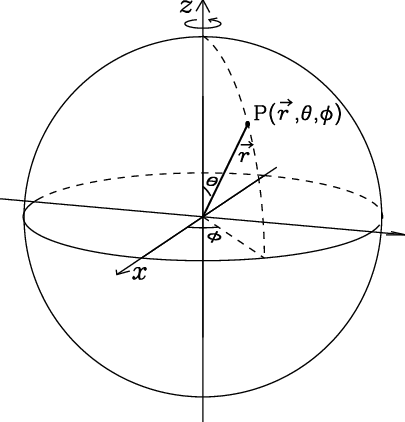
\includegraphics[scale=0.155]{figures/The-spherical-polar-coordinate-system}
      \caption{The spherical polar coordinate system\tiny\cite{sphericalpolarcoordinate}}
    \end{figure}
  \end{columns}
  }%
\end{frame}

\begin{frame}{State of Single-Qubit System\tiny\cite{blochsphere}}
  \framesubtitle{Bloch Sphere}
  {\tiny
  Following is derived already:
  \begin{align*}
    \ket{\psi} &= \cos\theta'\ket{0}+e^{i\phi}\sin\theta'\ket{1} .
  \end{align*}
  When $\theta'=0$, $\ket{\psi}=\ket{0}$; when $\theta'=\frac{\pi}2$, $\ket{\psi}=e^{i\phi}\ket{1}$.
  This suggests there is redundancy in sphere model above.
  Looking at the opposite point of $\ket{\psi}$ on the sphere:
  \begin{align*}
    \ket{\psi'} &= \cos(\pi-\theta')\ket{0}+e^{i(\pi+\phi)}\sin(\pi-\theta')\ket{1} \\
     &= -\cos(\theta')\ket{0}+e^{i\pi}e^{i\phi}\sin\theta'\ket{1} \\
     &= -\cos(\theta')\ket{0}-e^{i\phi}\sin\theta'\ket{1} \\
     &= -\ket{\psi} .
  \end{align*}
  It has only a global phase difference. So a hemisphere is able to represent a qubit. Finally a qubit can be modeled as a \textbf{Bloch Sphere}:
  \begin{align*}
    \ket{\psi} &= \cos(\frac{\theta}2)\ket{0}+e^{i\phi}\sin(\frac{\theta}2)\ket{1}
  \end{align*}
  where $0\leqslant\theta\leqslant\pi$, $0\leqslant\phi\leqslant2\pi$.
  }%
\end{frame}

\begin{frame}{Special States on the Bloch Sphere}
  {\tiny
  $\ket{\psi} = \cos(\frac{\theta}2)\ket{0}+e^{i\phi}\sin(\frac{\theta}2)\ket{1}$, where $0\leqslant\theta\leqslant\pi$, $0\leqslant\phi\leqslant2\pi$.
  \begin{figure}
    \centering
    \begin{subfigure}[b]{0.5\textwidth}
      \centering
      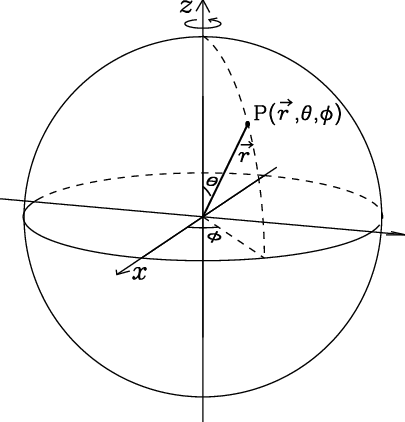
\includegraphics[scale=0.2]{figures/The-spherical-polar-coordinate-system}
      \caption{The spherical polar coordinate system\tiny\cite{sphericalpolarcoordinate}}
    \end{subfigure}
    \hfill
    \begin{subfigure}[b]{0.5\textwidth}
      \centering
      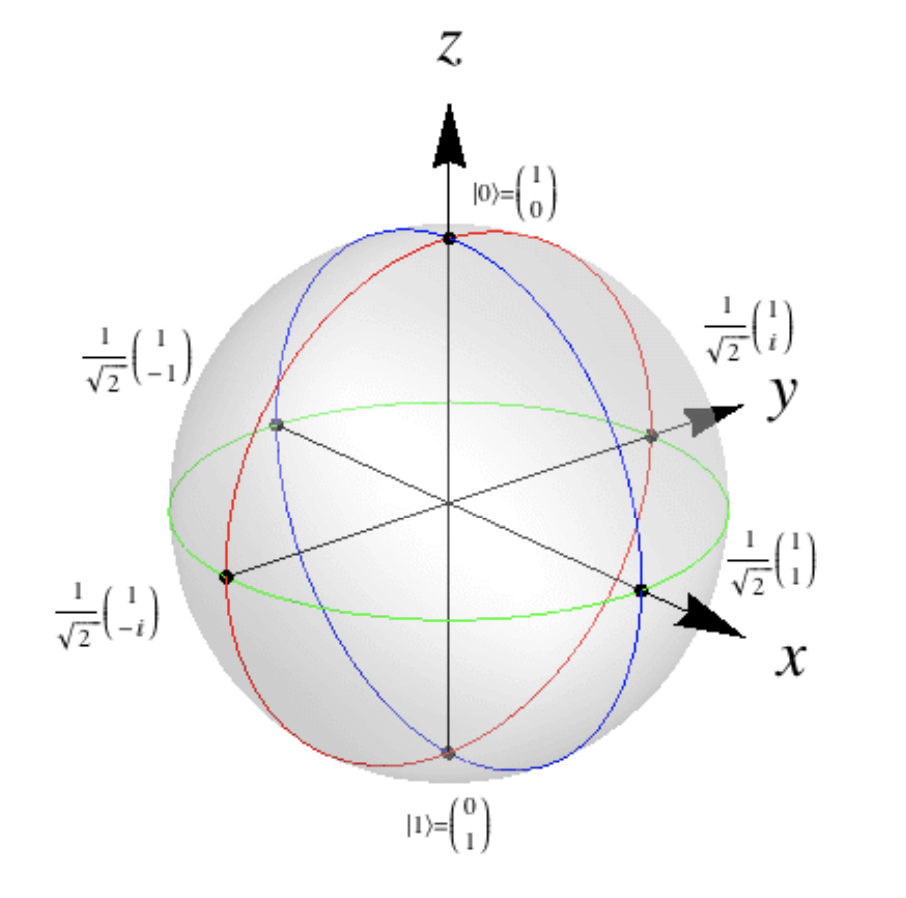
\includegraphics[scale=0.24]{figures/singlequbitstates}
      \caption{The special single qubit states\tiny\cite{singlequbitstates}}
    \end{subfigure}
    \caption{The Block Sphere}
  \end{figure}
  \begin{align*}
  \ket0 &\mapsto \theta = 0                     & \ket1 &\mapsto \theta = \pi \\
  \ket+ &\mapsto \theta = \frac{\pi}2, \phi = 0 & \ket- &\mapsto \theta = \frac{\pi}2, \phi = \pi \\
  \ket{i} &\mapsto \theta = \frac{\pi}2, \phi = \frac{\pi}2 & \ket{-i} &\mapsto \theta = \frac{\pi}2, \phi = \frac{3\pi}2
  \end{align*}
  }%
\end{frame}

\subsection{Rotation on the Bloch Sphere}
\begin{frame}{The Exponential Operator\tiny\cite{rotationsonblochsphere}}
  {\tiny
    Suppose $f(x)$ has a power series $f(x) = \sum_{i=0}^{\infty}c_ix^n$, and define $f(\mathbf{A})$ as:
    \begin{align*}
    f(\mathbf{A}) \equiv c_0\mathbf{I} + c_1\mathbf{A} + c_2\mathbf{A^2} + c_3\mathbf{A^3} + \dots
    \end{align*}
    With Taylor Series:
    \begin{align*}
      \sin{x} &= x - \frac{x^3}{3!} + \frac{x^5}{5!} - \dots \frac{(-1)^kx^{2k+1}}{(2k+1)!}\ \dots \\
      \cos{x} &= 1 - \frac{x^2}{2!} + \frac{x^4}{4!} - \dots \frac{(-1)^kx^{2k}}{(2k)!}\ \dots \\
      e^{ix} &= 1 + \frac{ix}{1!} + \frac{i^2x^2}{2!} + \frac{i^3x^3}{3!}+ \frac{i^4x^4}{4!} + \frac{i^5x^5}{5!} + \dots \\
             &= (1 - \frac{x^2}{2!} + \frac{x^4}{4!} - \dots) + i(x - \frac{x^3}{3!} + \frac{x^5}{5!} - \dots) \\
             &= \cos{x} + i\sin{x}
    \end{align*}
    In case that $\mathbf{A}^2=\mathbf{I}$:
    \begin{align*}
      e^{i\alpha\mathbf{A}} &= \mathbf{I}
                                 + \frac{i\alpha\mathbf{A}}{1!}
                                 + \frac{i^2(\alpha\mathbf{A})^2}{2!}
                                 + \frac{i^3(\alpha\mathbf{A})^3}{3!}
                                 + \frac{i^4(\alpha\mathbf{A})^4}{4!}
                                 + \dots \\
                            &= \cos(\alpha)\mathbf{I} + i\sin(\alpha)\mathbf{A}
    \end{align*}
  }%
\end{frame}

\begin{frame}{The Pauli Matrices and the Rotation Operators\tiny\cite{rotationsonblochsphere}}
  {\tiny
    Given a qubit:
    \begin{align*}
      \ket{\psi} = \cos(\frac{\theta}2)\ket{0}+e^{i\phi}\sin(\frac{\theta}2)\ket{1} &= \begin{bmatrix}\cos{\frac{\theta}2} \\ e^{i\phi}\sin{\frac{\theta}2} \end{bmatrix}
    \end{align*}
    where $0\leqslant\theta\leqslant\pi$, $0\leqslant\phi\leqslant2\pi$, and the exponential operator defined above:
    \begin{align*}
      e^{i\alpha\mathbf{A}} = \cos(\alpha)\mathbf{I} + i\sin(\alpha)\mathbf{A}
    \end{align*}
    Define operators $R_x(\alpha)$, $R_y(\alpha)$ and $R_z(\alpha)$:
    \begin{align*}
      R_x(\alpha) &\equiv \cos\frac{\alpha}2\mathbf{I} - i\sin\frac{\alpha}2
                                                                     \begin{bmatrix}
                                                                       1 & 0 \\
                                                                       0 & 1
                                                                     \end{bmatrix}
                  &&= e^{-i\frac{\alpha}2\mathbf{X}}
                  &&= \cos\frac{\alpha}2\mathbf{I} - i\sin\frac{\alpha}2 \mathbf{X}
                  &&=\begin{bmatrix}
                    \cos\frac{\alpha}2 & -i\sin\frac{\alpha}2 \\
                    -i\sin\frac{\alpha}2 & \cos\frac{\alpha}2
                    \end{bmatrix} \\
      R_y(\alpha) &\equiv \cos\frac{\alpha}2\mathbf{I} - i\sin\frac{\alpha}2
                                                                     \begin{bmatrix}
                                                                       0 & -i \\
                                                                       i & 0
                                                                     \end{bmatrix}
                  &&= e^{-i\frac{\alpha}2\mathbf{Y}}
                  &&= \cos\frac{\alpha}2\mathbf{I} - i\sin\frac{\alpha}2 \mathbf{Y}
                  &&=\begin{bmatrix}
                    \cos\frac{\alpha}2 & -\sin\frac{\alpha}2 \\
                    \sin\frac{\alpha}2 & \cos\frac{\alpha}2
                    \end{bmatrix} \\
      R_z(\alpha) &\equiv \cos\frac{\alpha}2\mathbf{I} - i\sin\frac{\alpha}2
                                                                     \begin{bmatrix}
                                                                       1 & 0 \\
                                                                       0 & -1 
                                                                     \end{bmatrix}
                  &&= e^{-i\frac{\alpha}2\mathbf{Z}}
                  &&= \cos\frac{\alpha}2\mathbf{I} - i\sin\frac{\alpha}2 \mathbf{Z}
                  &&=\begin{bmatrix}
                    e^{-i\frac{\alpha}2} & 0 \\
                    0 & e^{i\frac{\alpha}2}
                    \end{bmatrix} \\
    \end{align*}
    The $\mathbf{X}$, $\mathbf{Y}$, and $\mathbf{Z}$ are Pauli Matrices.
  }%
\end{frame}

\begin{frame}{An Example of Rotation\tiny\cite{rotationsonblochsphere}}
  {\tiny
    Rotate $\ket\psi$ about z-axis by angle of $\alpha$ on the Bloch Sphere:
  \begin{align*}
    R_z(\alpha)\ket{\psi} &= \begin{bmatrix}
                                e^{-i\frac{\alpha}2} & 0 \\
                                0                    & e^{i\frac{\alpha}2}
                              \end{bmatrix}
                              \begin{bmatrix}
                                \cos{\frac{\theta}2} \\
                                e^{i\phi}\sin{\frac{\theta}2}
                              \end{bmatrix} \\
                          &= \begin{bmatrix}
                               e^{-i\frac{\alpha}2}\cos{\frac{\theta}2} \\
                               e^{i\frac{\alpha}2}\sin{\frac{\theta}2} 
                             \end{bmatrix} \\
     e^{i\frac{\alpha}2}R_z(\alpha)\ket{\psi}
                          &= \begin{bmatrix}
                               \cos{\frac{\theta}2} \\
                               e^{i\alpha}e^{i\phi}\sin{\frac{\theta}2}
                             \end{bmatrix} \\
    \\
    R_x(\alpha)\ket{\psi} &= \begin{bmatrix}
                              \cos\frac{\alpha}2 & -i\sin\frac{\alpha}2 \\
                              -i\sin\frac{\alpha}2 & \cos\frac{\alpha}2
                             \end{bmatrix}
                             \begin{bmatrix}
                               \cos{\frac{\theta}2} \\
                               e^{i\phi}\sin{\frac{\theta}2}
                             \end{bmatrix} \\
                             &= \begin{bmatrix}
                               \cos\frac{\alpha}2 \cos\frac{\theta}2 - i e^{i\phi} \sin\frac{\alpha}2 \sin\frac{\theta}2 \\
                               -i \sin\frac{\alpha}2 \cos\frac{\theta}2 + e^{i\phi} \cos\frac{\alpha}2 \sin\frac{\theta}2
                                \end{bmatrix} \\
                             &= \dots
  \end{align*}
  }%
\end{frame}

\begin{frame}{The Density Operator\tiny\cite{rotationsonblochsphere}}
  {\tiny
  Another representation of a qubit $\ket{\psi}$:
    \begin{align*}
      \rho &= \ket{\psi} \otimes \bra{\psi} = \ket{\psi} \otimes \ket{\psi}^{\dagger} \\
           &= \begin{bmatrix}
                \cos{\frac{\theta}2} \\
                e^{i\phi}\sin{\frac{\theta}2}
              \end{bmatrix}
              \otimes
              \begin{bmatrix}
                \cos{\frac{\theta}2} & e^{-i\phi}\sin{\frac{\theta}2}
              \end{bmatrix} \\
           &= \begin{bmatrix}
                \cos^2{\frac{\theta}2}                            & e^{-i\phi}\cos{\frac{\theta}2}\sin{\frac{\theta}2} \\
                e^{i\phi}\cos{\frac{\theta}2}\sin{\frac{\theta}2} & \sin^2{\frac{\theta}2}
              \end{bmatrix} \\
           &= \begin{bmatrix}
                \frac{1+\cos{\theta}}2                       & (\cos{\phi}-i\sin{\phi})\frac{\sin\theta}2 \\
                (\cos{\phi}+i\sin{\phi})\frac{\sin\theta}2   & \frac{1-\cos{\theta}}2
              \end{bmatrix} \\
           &= \frac{1}2
              \begin{pmatrix}
                \begin{bmatrix}
                  1 & 0 \\
                  0 & 1
                \end{bmatrix}
                +
                \cos\phi\sin\theta
                \begin{bmatrix}
                  0 & 1 \\
                  1 & 0
                \end{bmatrix}
                +
                \sin\phi\sin\theta
                \begin{bmatrix}
                  0 & -i \\
                  i & 0
                \end{bmatrix}
                +
                \cos\theta
                \begin{bmatrix}
                  1 & 0 \\
                  0 & -1 
                \end{bmatrix}
              \end{pmatrix} \\
            &= \frac{1}2(\mathbf{I} + \mathbf{X}\cos\phi\sin\theta + \mathbf{Y}\sin\phi\sin\theta + \mathbf{Z}\cos\theta) \\
            &= \frac{1}2(\mathbf{I} + (\mathbf{X}, \mathbf{Y}, \mathbf{Z}) \cdot (r_x, r_y, r_z)) \\
            &= \frac{1}2 ( \mathbf{I} + \overrightarrow{\sigma} \cdot \overrightarrow{\mathbf{r}}_{\rho} )
    \end{align*}
  }%
\end{frame}

\begin{frame}{Rotation with the Density Operator - I\tiny{\cite{rotationsonblochsphere}}}
  {\tiny
    For rotation $R_z(\alpha)$:
    \begin{columns}
    \column{0.7\textwidth}
    \begin{align*}
      \rho' &= R_z(\alpha)\ket{\psi} \otimes (R_z(\alpha)\ket{\psi})^{\dagger} \\
            &= R_z(\alpha)(\ket{\psi} \otimes \bra{\psi})R_z(\alpha)^{\dagger} \\
            &= R_z(\alpha) \rho R_z(\alpha)^{\dagger} \\
            &= \frac{1}2(\mathbf{I}  + r_x R_z(\alpha) \mathbf{X} R_z(\alpha)^{\dagger}
                                     + r_y R_z(\alpha) \mathbf{Y} R_z(\alpha)^{\dagger} 
                                     + r_z R_z(\alpha) \mathbf{Z} R_z(\alpha)^{\dagger} \\
      \\
      R_z(\alpha) \mathbf{X} R_z(\alpha)^{\dagger}
            &=    \begin{pmatrix} \cos\frac{\alpha}2\mathbf{I} - i\sin\frac{\alpha}2 \mathbf{Z} \end{pmatrix}
                  \mathbf{X}
                  \begin{pmatrix} \cos\frac{\alpha}2\mathbf{I} + i\sin\frac{\alpha}2 \mathbf{Z} \end{pmatrix} \\
            &=    \cos^2\frac{\alpha}2 \mathbf{X}
                + i\sin\frac{\alpha}2 \cos\frac{\alpha}2 \mathbf{X}\mathbf{Z}
                - i\sin\frac{\alpha}2 \cos\frac{\alpha}2 \mathbf{Z}\mathbf{X}
                + \sin^2\frac{\alpha}2 \mathbf{Z}\mathbf{X}\mathbf{Z} \\
            &=    \begin{pmatrix} \cos^2\frac{\alpha}2 -  \sin^2\frac{\alpha}2 \end{pmatrix} \mathbf{X}
                + 2 \sin\frac{\alpha}2 \cos\frac{\alpha}2 \mathbf{Y} \\
            &= \cos\alpha \mathbf{X} + \sin\alpha \mathbf{Y} \\
      R_z(\alpha) \mathbf{Y} R_z(\alpha)^{\dagger}
            &=    \cos\alpha \mathbf{Y} - \sin\alpha \mathbf{X} \\
      R_z(\alpha) \mathbf{Z} R_z(\alpha)^{\dagger}
            &=    \begin{pmatrix} \cos\frac{\alpha}2\mathbf{I} - i\sin\frac{\alpha}2 \mathbf{Z} \end{pmatrix}
                  \mathbf{Z}
                  \begin{pmatrix} \cos\frac{\alpha}2\mathbf{I} + i\sin\frac{\alpha}2 \mathbf{Z} \end{pmatrix} \\
            &=    \cos^2\frac{\alpha}2 \mathbf{Z}
                + i\sin\frac{\alpha}2 \cos\frac{\alpha}2 \mathbf{Z}\mathbf{Z}
                - i\sin\frac{\alpha}2 \cos\frac{\alpha}2 \mathbf{Z}\mathbf{Z}
                + \sin^2\frac{\alpha}2 \mathbf{Z}\mathbf{Z}\mathbf{Z} \\
            &=    \mathbf{Z} \\
      \\
      \rho' &= \frac{1}2 ( \mathbf{I} + \overrightarrow{\sigma} \cdot \overrightarrow{\mathbf{r}}_{\rho'} )
            , where \overrightarrow{\mathbf{r}}_{\rho'} =
              \begin{bmatrix}
                \cos\alpha & -\sin\alpha & 0 \\
                \sin\alpha & \cos\alpha  & 0 \\
                0          & 0           & 1
              \end{bmatrix}
              \overrightarrow{\mathbf{r}}_{\rho}
    \end{align*}
    \column{0.3\textwidth}
    \setbeamerfont{block title}{size=\tiny}
    \begin{block}{The Algebra of the Pauli Matrices}
      $\mathbf{X}^2 = \mathbf{Y}^2 = \mathbf{Z}^2 = -i\mathbf{XYZ} = \mathbf{I}$ \\
      $\mathbf{XY} = -\mathbf{YX} = i\mathbf{Z}$ \\
      $\mathbf{YZ} = -\mathbf{ZY} = i\mathbf{X}$ \\
      $\mathbf{ZX} = -\mathbf{XZ} = i\mathbf{Y}$
    \end{block}
    \end{columns}
  }%
\end{frame}

\begin{frame}{Rotation with the Density Operator - II}
  {\tiny
    For rotation $R_x(\alpha)$:
    \begin{align*}
      \rho' &= R_x(\alpha) \rho R_x(\alpha)^{\dagger} \\
            &= \frac{1}2(\mathbf{I}  + r_x R_x(\alpha) \mathbf{X} R_x(\alpha)^{\dagger}
                                     + r_y R_x(\alpha) \mathbf{Y} R_x(\alpha)^{\dagger} 
                                     + r_z R_x(\alpha) \mathbf{Z} R_x(\alpha)^{\dagger} \\
      \\
      R_x(\alpha) \mathbf{X} R_x(\alpha)^{\dagger}
            &=  \begin{pmatrix} \cos\frac{\alpha}2\mathbf{I} - i\sin\frac{\alpha}2 \mathbf{X} \end{pmatrix}
                \mathbf{X}
                \begin{pmatrix} \cos\frac{\alpha}2\mathbf{I} + i\sin\frac{\alpha}2 \mathbf{X} \end{pmatrix} \\
            &=    \cos^2\frac{\alpha}2 \mathbf{X}
                + i\sin\frac{\alpha}2 \cos\frac{\alpha}2 \mathbf{X}\mathbf{X}
                - i\sin\frac{\alpha}2 \cos\frac{\alpha}2 \mathbf{X}\mathbf{X}
                + \sin^2\frac{\alpha}2 \mathbf{X}\mathbf{X}\mathbf{X} \\
            &= X \\
      R_x(\alpha) \mathbf{Y} R_x(\alpha)^{\dagger}
            &=  \begin{pmatrix} \cos\frac{\alpha}2\mathbf{I} - i\sin\frac{\alpha}2 \mathbf{X} \end{pmatrix}
                \mathbf{Y}
                \begin{pmatrix} \cos\frac{\alpha}2\mathbf{I} + i\sin\frac{\alpha}2 \mathbf{X} \end{pmatrix} \\
            &=    \cos^2\frac{\alpha}2 \mathbf{Y}
                + i\sin\frac{\alpha}2 \cos\frac{\alpha}2 \mathbf{Y}\mathbf{X}
                - i\sin\frac{\alpha}2 \cos\frac{\alpha}2 \mathbf{X}\mathbf{Y}
                + \sin^2\frac{\alpha}2 \mathbf{X}\mathbf{Y}\mathbf{X} \\
            &=    \cos^2\frac{\alpha}2 \mathbf{Y}
                + \sin\frac{\alpha}2 \cos\frac{\alpha}2 \mathbf{Z}
                + \sin\frac{\alpha}2 \cos\frac{\alpha}2 \mathbf{Z}
                - \sin^2\frac{\alpha}2 \mathbf{Y} \\
            &=    \cos\alpha \mathbf{Y} + \sin\alpha \mathbf{Z} \\
      R_z(\alpha) \mathbf{Z} R_z(\alpha)^{\dagger}
            &=    \cos\alpha \mathbf{Z} - \sin\alpha \mathbf{Y} \\
      \\
      \rho' &= \frac{1}2 ( \mathbf{I} + \overrightarrow{\sigma} \cdot \overrightarrow{\mathbf{r}}_{\rho'} )
            , where \overrightarrow{\mathbf{r}}_{\rho'} =
              \begin{bmatrix}
                1 & 0          & 0 \\
                0 & \cos\alpha & -\sin\alpha \\
                0 & \sin\alpha & \cos\alpha \\
              \end{bmatrix}
              \overrightarrow{\mathbf{r}}_{\rho}
    \end{align*}
  }%
\end{frame}

\begin{frame}{Rotation with the Density Operator - III}
  {\tiny
    For rotation $R_y(\alpha)$:
    \begin{align*}
      \rho' &= R_y(\alpha) \rho R_y(\alpha)^{\dagger} \\
            &= \frac{1}2(\mathbf{I}  + r_x R_y(\alpha) \mathbf{X} R_y(\alpha)^{\dagger}
                                     + r_y R_y(\alpha) \mathbf{Y} R_y(\alpha)^{\dagger} 
                                     + r_z R_y(\alpha) \mathbf{Z} R_y(\alpha)^{\dagger} \\
      \\
      R_y(\alpha) \mathbf{X} R_y(\alpha)^{\dagger}
            &=    \begin{pmatrix} \cos\frac{\alpha}2\mathbf{I} - i\sin\frac{\alpha}2 \mathbf{Y} \end{pmatrix}
                  \mathbf{X}
                  \begin{pmatrix} \cos\frac{\alpha}2\mathbf{I} + i\sin\frac{\alpha}2 \mathbf{Y} \end{pmatrix} \\
            &=    \cos^2\frac{\alpha}2 \mathbf{X}
                + i\sin\frac{\alpha}2 \cos\frac{\alpha}2 \mathbf{X}\mathbf{Y}
                - i\sin\frac{\alpha}2 \cos\frac{\alpha}2 \mathbf{Y}\mathbf{X}
                + \sin^2\frac{\alpha}2 \mathbf{Y}\mathbf{X}\mathbf{Y} \\
            &=    \cos^2\frac{\alpha}2 \mathbf{X}
                - \sin\frac{\alpha}2 \cos\frac{\alpha}2 \mathbf{Z}
                - \sin\frac{\alpha}2 \cos\frac{\alpha}2 \mathbf{Z}
                - \sin^2\frac{\alpha}2 \mathbf{X} \\
            &=    \cos\alpha \mathbf{X} - \sin\alpha \mathbf{Z} \\
      R_y(\alpha) \mathbf{Y} R_y(\alpha)^{\dagger}
            &= Y \\
      R_y(\alpha) \mathbf{Z} R_y(\alpha)^{\dagger}
            &=    \begin{pmatrix} \cos\frac{\alpha}2\mathbf{I} - i\sin\frac{\alpha}2 \mathbf{Y} \end{pmatrix}
                  \mathbf{Z}
                  \begin{pmatrix} \cos\frac{\alpha}2\mathbf{I} + i\sin\frac{\alpha}2 \mathbf{Y} \end{pmatrix} \\
            &=    \cos^2\frac{\alpha}2 \mathbf{Z}
                + i\sin\frac{\alpha}2 \cos\frac{\alpha}2 \mathbf{Z}\mathbf{Y}
                - i\sin\frac{\alpha}2 \cos\frac{\alpha}2 \mathbf{Y}\mathbf{Z}
                + \sin^2\frac{\alpha}2 \mathbf{Y}\mathbf{Z}\mathbf{Y} \\
            &=    \cos^2\frac{\alpha}2 \mathbf{Z}
                + \sin\frac{\alpha}2 \cos\frac{\alpha}2 \mathbf{X}
                + \sin\frac{\alpha}2 \cos\frac{\alpha}2 \mathbf{X}
                - \sin^2\frac{\alpha}2 \mathbf{Z} \\
            &= \cos\alpha \mathbf{Z} + \sin\alpha \mathbf{X} \\
      \\
      \rho' &= \frac{1}2 ( \mathbf{I} + \overrightarrow{\sigma} \cdot \overrightarrow{\mathbf{r}}_{\rho'} )
            , where \overrightarrow{\mathbf{r}}_{\rho'} =
              \begin{bmatrix}
                \cos\alpha  & 0 & \sin\alpha \\
                0           & 1 & 0 \\
                -\sin\alpha & 0 & \cos\alpha \\
              \end{bmatrix}
              \overrightarrow{\mathbf{r}}_{\rho}
    \end{align*}
  }%
\end{frame}

\section{Multiple-Qubit System}
\begin{frame}
  Multiple-Qubit System
\end{frame}

\begin{frame}{State Space of 2-Qubit System}
  {\tiny
  All possible states of a single-qubit system is viewed as a two-dimensional complex vector space.\\
  All possible states of a 2-qubit system is viewed as the tensor product $\otimes$ of two such vector spaces.
  This tensor product is a vecor space as well. Its dimension is $2^2$.\\
  Let $\mathbf{V}$ and $\mathbf{W}$ be two-dimensional complex vector spaces with
  bases $A=\{\ket{\alpha_1}, \ket{\alpha_2}\}$ and $B=\{\ket{\beta_1}, \ket{\beta_2}\}$ respectively. \\
  One basis of $\mathbf{V} \otimes \mathbf{W}$ is:
  \begin{align*}
    \{\ket\alpha_1 \otimes \ket\beta_1,
       \ket\alpha_1 \otimes \ket\beta_2,
       \ket\alpha_2 \otimes \ket\beta_1,
       \ket\alpha_2 \otimes \ket\beta_2 \}
  \end{align*}
  With standard basis on both vector spaces, one basis of the tensor product is:
  \begin{align*}
    \{\ket0 \otimes \ket0, \ket0 \otimes \ket1, \ket1 \otimes \ket0, \ket1 \otimes \ket1 \}
    &= \{\ket{00}, \ket{01}, \ket{10}, \ket{11} \} \\
    &= \{
      \begin{bmatrix} 1 \\ 0 \\ 0 \\ 0 \end{bmatrix},
      \begin{bmatrix} 0 \\ 1 \\ 0 \\ 0 \end{bmatrix},
      \begin{bmatrix} 0 \\ 0 \\ 1 \\ 0 \end{bmatrix},
      \begin{bmatrix} 0 \\ 0 \\ 0 \\ 1 \end{bmatrix}
    \}
  \end{align*}
  Examples: \\
  Let state $\ket{v}=a_1\ket0 + a_2\ket1$ and state $\ket{w}=b_1\ket0 + b_2\ket1$, the tensor product of these two states is:
  \begin{align*}
  a_1b_1\ket{00} + a_1b_2\ket{01} + a_2b_1\ket{10} + a_2b_2\ket{11}
  \end{align*}
  Can you find $a_1$, $a_2$, $b_1$, and $b_2$ which satisfy following?
  \begin{align*}
  (a_1\ket0 + a_2\ket1) \otimes (b_1\ket0 + b_2\ket1) = \frac{1}{\sqrt2}(\ket{00} + \ket{11})
  \end{align*}
  It turns out that some states of 2-qubit quantum system cannot be described in terms of the state of two separate single-qubit systems.
  These states stand for \textbf{entanglement} of the 2-qubit quantum system.
  }%
\end{frame}

\begin{frame}
  Not give up yet.
  \par
  To be continued\dots
\end{frame}

\begin{frame}{Rotation on the Bloch Sphere}
  \framesubtitle{Spectual Decomposition, Operator Functions and Power Series}
  {\tiny
    Suppose $\mathbf{u}_1$, $\dots$, $\mathbf{u}_n$ are eigenvectors of $\mathbf{A}$.
    $\lambda_1$, $\dots$, $\lambda_n$ are corresponding eigenvalues of these eigenvectors.
    \begin{align*}
      \mathbf{A} &= \begin{bmatrix}
                      \mathbf{u}_1 & \dots & \mathbf{u}_n
                    \end{bmatrix}
                    \begin{bmatrix}
                      \lambda_1 &  & 0 \\
                      & \ddots & \\
                      0 & &  \lambda_n
                    \end{bmatrix}
                    \begin{bmatrix}
                      \mathbf{u}^{T}_1 \\
                      \vdots \\
                      \mathbf{u}^{T}_n
                    \end{bmatrix} \\
                  &=   \lambda_1\mathbf{u}_1\mathbf{u}^{T}_1
                     + \lambda_2\mathbf{u}_2\mathbf{u}^{T}_2
                     + \dots
                     + \lambda_n\mathbf{u}_n\mathbf{u}^{T}_n \\
                     &= \sum\limits_{i=1}^n \lambda_i\ket{u_i}\bra{u_i}
    \end{align*}
  }%
\end{frame}

\begin{frame}{Review math knowledge we learned in school}
  {\tiny
    \setbeamerfont{block title}{size=\tiny}
    \begin{block}{The Invertible Matrix Theorem for $A^{-1}$}
      $\begin{bmatrix}A&I\end{bmatrix}$ is row equivalent to $\begin{bmatrix}I&A^{-1}\end{bmatrix}$  \\
      $Ax=e_1, Ax=e_2,  \dots, Ax=e_n$ \\
      $A$ is row equivalent to the $n{\times}n$ identity matrix \\
      The equation $Ax=0$ has only the trivial solution
    \end{block}
  }%
\end{frame}


\end{document}
